\section{Einleitung und Motivation}
\autor{Medjen Izairi}
Autonomes Fahren, auch als selbstfahrende oder autonome Fahrzeugtechnologie bezeichnet, repräsentiert einen wegweisenden Fortschritt im Bereich der Mobilität. Bei dieser Technologie übernimmt das Fahrzeug die Steuerung, Navigation und oft auch die Entscheidungsfindung, ohne direkten menschlichen Eingriff. Im Zeitalter des autonomen Fahrens spielt die effiziente Steuerung des Verhaltens autonomer Fahrzeuge eine zentrale Rolle, um sichere und sozialverträgliche Interaktionen im Straßenverkehr zu gewährleisten. Die Herausforderung besteht darin, dass autonom agierende Fahrzeuge in Echtzeit komplexe Entscheidungen treffen müssen, um sich flexibel an wechselnde Verkehrssituationen anzupassen. In diesem Kontext gewinnen Verhaltensbäume (Behavior Trees) als ein flexibler und modularer Ansatz für die Entscheidungsfindung in autonom gesteuerten Systemen zunehmend an Bedeutung. Diese ermöglichen es, das Verhalten von autonomen Fahrzeugen auf eine übersichtliche und hierarchische Weise zu organisieren, was besonders in dynamischen und unvorhersehbaren Verkehrsszenarien von entscheidendem Vorteil ist. Das System kann in Echtzeitsituationen, in denen autonome Fahrzeuge sich schnell an veränderte Umgebungen anpassen müssen, effektiv und schnell auf neue Informationen reagieren Diese Fähigkeit erweist sich als entscheidend, insbesondere in Situationen mit hoher Sicherheitsrelevanz. In der bisherigen Softwarearchitektur wurde ein Switch Case (Fallunterscheidungen) als grundlegendes Entscheidungssystem verwendet. Obwohl das System anfangs funktional war, wies es einige Nachteile auf. Mit zunehmender Anzahl von möglichen Verhaltensszenarien stieg die Komplexität des Codes. Dies erschwerte nicht nur die Entwicklung, sondern auch die Wartung und Fehlerbehebung. In Echtzeitszenarien führte dies zu zahlreichen Verzögerungen und Schwierigkeiten, angemessen in Echtzeit zu reagieren. Daher haben wir uns für Behavior Trees entschieden, als eine effiziente Möglichkeit, die Komplexität unseres autonomen Fahrzeug-Systems zu bewältigen. 
\begin{figure}
    \centering
    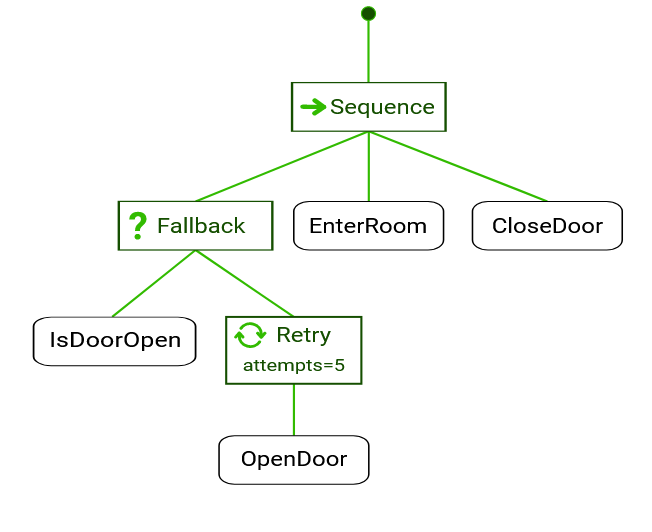
\includegraphics[width=0.45\linewidth]{Pictures/grafik.png}
    \caption{Behavior Tree}
    \cite{behaviortree}
    \label{fig:enter-label}
\end{figure}




